\documentclass[10pt,a4paper,final,conference]{IEEEtran}
\title{Survey of Hybrid Vanet Design for Provisioning Infotaintment Appplication}
\usepackage{amsmath}
\usepackage{graphicx}

%Packages For flowcharts
\usepackage{tikz}
\usetikzlibrary{shapes.geometric, arrows}
% Create a node start/stop block with rounded corners
\tikzstyle{startstop} = [rectangle,rounded corners,minimum width=3cm,
minimum height=1cm,text centered,draw = black]
% Create a input/output box called io
\tikzstyle{io} = [trapezium, trapezium left angle=70,
trapezium right angle=110, minimum width=3cm, minimum height=1cm,
text centered,draw = black]
% Create a processing block called process
\tikzstyle{process} = [rectangle, minimum width=3cm, minimum height=1cm,
text centered,draw = black]
% Create a decision box and name it as decision
\tikzstyle{decision} = [diamond, minimum width=3cm, minimum height=1cm,
text centered, draw=black]
% Create arrow 
\tikzstyle{arrow} = [thick,->,>=stealth]

\author{
	
	\IEEEauthorblockN{Abhilash T}
	\IEEEauthorblockA{Dept. of CSE\\
		AMC Engineering College\\
		Bangalore,India
	}
	
	\and
	
	\IEEEauthorblockN{Chandrashekar}
	\IEEEauthorblockA{Dept. of CSE\\
		AMC Engineering College\\
		Bangalore,India
	}
	
	\and
	
	\IEEEauthorblockN{Shalini S}
	\IEEEauthorblockA{Dept. of CSE\\
		AMC Engineering College\\
		Bangalore,India
	}
	
}

%\author{
%		\IEEEauthorblockN{Michael Shell\IEEEauthorrefmark{1}, Homer Simpson\IEEEauthorrefmark{2}, James K
%			irk\IEEEauthorrefmark{3}, Montgomery Scott\IEEEauthorrefmark{3} and Eldon Tyrell\IEEEauthorrefmark{4}}
%	
%		\IEEEauthorblockA{\IEEEauthorrefmark{1}School of Electrical and Computer Engineering\\
%			Georgia Institute of Technology, Atlanta, Georgia 30332--0250\\
%			Email: mshell@ece.gatech.edu}
%		\IEEEauthorblockA{\IEEEauthorrefmark{2}Twentieth Century Fox, Springfield, USA\\
%			Email: homer@thesimpsons.com}
%		\IEEEauthorblockA{\IEEEauthorrefmark{3}Starfleet Aca
%		demy, San Francisco, California 96678-2391\\
%		Telephone: (800) 555--1212, Fax: (888) 555--1212}
%		\IEEEauthorblockA{\IEEEauthorrefmark{4}Tyrell Inc.,
%			123 Replicant Street, Los Angeles, California 90210
%			--4321}}



\begin{document}
	\maketitle
	\begin{abstract}
		The purpose of this paper is to present a design of a
		home security system which is economical, energy efficient and
		portable. The system provides the user complete control over its
		functionalities. The setup of the home security system involves
		the use of a Raspberry Pi 3 model B to which a Passive Infrared
		Sensor (PIR sensor) and a webcam are connected. The Raspberry
		Pi 3 model B uses a 1.2 GHz quad-core ARM Cortex-A53 for
		processing, while the PIR sensor is used to detect motion and the
		webcam is used to perform face detection and image capturing
		processes using OpenCV image processing library and Python
		programming language.
	\end{abstract}
\vspace{0.5cm}
\begin{IEEEkeywords}
	Raspberry Pi 3 model B, PIR Sensor, ARM Cortex-
	A53 processor, Python, SMTP, MIME, OpenCV, IoT.
\end{IEEEkeywords}

\section{Introduction}
Home security Eq.\ref{eq:1} systems have become predominant in the
everyday life of modern society. Home security is a concept
that consists of using hardware and software technologies to
implement security systems that would secure and protect the
assets within its secure environment. The advent of Internet of
things (IoT)  has further improved Eq.\ref{eq:simple}the features provided by
security systems. Based on a report by MarketsAndMarkets 
the security solutions market is expected to grow from USD
206.69 Billion in 2016 to USD 372.90 Billion by 2022. Hence
it has become crucial that security systems become less
expensive and more efficient.\\


\section{Equations}
\subsection{Single Equations}
$a+b+c$

\subsection{Subscripts and Superscripts}
\subsubsection{Subscripts}
$a_1 + a_2 + a_3 + \dots a_i$
\subsubsection{Superscripts}
$a^2 + b^2 +2a \cdot b $


\subsection{Inserting Equation}
\begin{equation}
	(a+b)^2 = a^2 +b^2 + 2 a \cdot b
	\label{eq:1}
\end{equation}
\begin{equation}
a = b+c-d+e-f
\label{eq:simple}
\end{equation}

\subsection{Inserting fractions}
\begin{equation}
f(x) = \frac{1}{x} +\frac{1}{x^2} +\frac{1}{x^3}
\end{equation}

\begin{equation}
\begin{pmatrix}
a&b\\
c&d
\end{pmatrix}
\end{equation}

\subsection{Mathematical Symbols}

\begin{equation}
5\alpha +6\beta +7 \gamma = 20
\end{equation}

\subsection{Inserting Summation and Integration}
\begin{eqnarray}
 \int\limits_0^1 x^2 + y^2 \ dx \\
 x= \sum_{i=0}^{z}2^iQ
\end{eqnarray}

\section{Inserting Figure}
\begin{figure}[h]
	\centering
	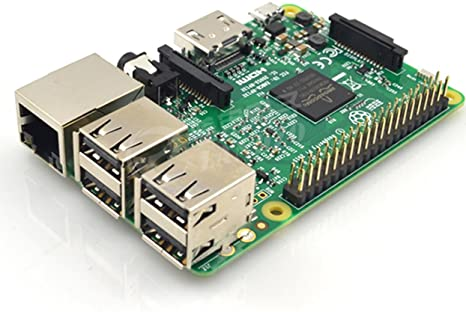
\includegraphics[width=0.5\linewidth,height=0.3\linewidth]{pi}
	\caption{Raspberry pi image side view}
	\label{fig:pi}
\end{figure}


\section{Inserting Tables}
\begin{table}[h]
\centering
\caption{Table of Subjects}
\begin{tabular}{|c|c|c|c|}
\hline
Sl.No & Subject & Subject Code & Number of students\\
\hline
1 & Computer Networks & 15CS365 & 56\\
\hline
2 & Operating Systems & 15CS461 & 45\\
\hline
\end{tabular}
\label{table:Subject}
\end{table}

\subsection{Inserting figures inside the table}
The images can be inserted inside the table using includegraphics without figure environment. The table shown in Table.\ref{tbl:img} has images. Table always appears on top unless mentioned
\begin{table}[h]
\centering
\caption{Table with figure}
\label{tbl:img}
\begin{tabular}{|c|c|c|}
	\hline
	SL.No. & National Symbol & Image\\
	\hline
	1 & Flower &  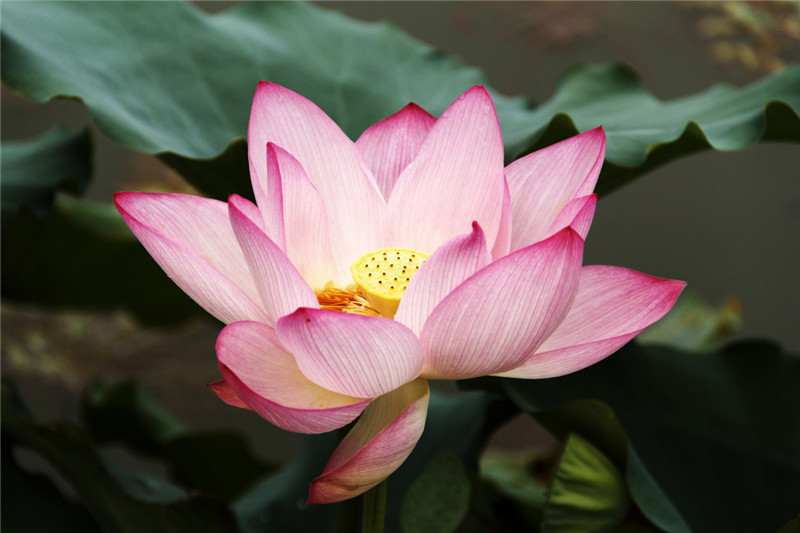
\includegraphics[width=0.1\linewidth,height=0.1\linewidth]{../Images/flower}\\
	\hline
	2 & Flag & 
	
\includegraphics[width=0.1\linewidth,height=0.1\linewidth]{../Images/flag}\\
	\hline
	3. & Emblem &
	
\includegraphics[width=0.1\linewidth,height=0.1\linewidth]{../Images/emblem}\\
	\hline
\end{tabular}
\end{table}

\subsection{Multicolumn table}
A multi column table can be created as shown in Table.\ref{table:statistics}
\begin{table}[!h]
	\centering
	\caption[Vital Statistics]{Regional Vital Statistics By State }
	\label{table:statistics}
	\begin{tabular}{|c|c|c|c|c|c|c|}
		\hline
		State & \multicolumn{3}{|c|}{Birth Rate}&\multicolumn{3}{|c|}{Natural growth Rate}\\
		\cline{2-7}
		& Total & Rural & Urban &Total & Rural & Urban\\
		\hline
		Karnataka & 19.2 &	20.2 &	17.5 &12.1	&12.1&	12.1\\
		\hline
		Delhi &	17.8 & 	19.7	&17.5	&13.6&	15.0	&13.4\\
		\hline
		Tamil Nadu	&15.9&	16.0&	15.8	&8.3	&7.8	&8.9\\
		\hline
		Kerala&	14.8&	14.8&	14.8& 7.8&	7.7	&8.1\\
		\hline		
	\end{tabular}
	
\end{table}

\section{Flowcharts}
Flowcharts can be included within figure environment
\begin{itemize}
	\item tikz package has to be included. % Refer to the top of the document to check for the needed packages
	\item The general flowchart is shown in Fig.\ref{fig:flowchart}.
	\item Include caption and label just like in figure environment.
\end{itemize}

\begin{figure}[!h]
\centering
% Can be scaled to fit in the alignment
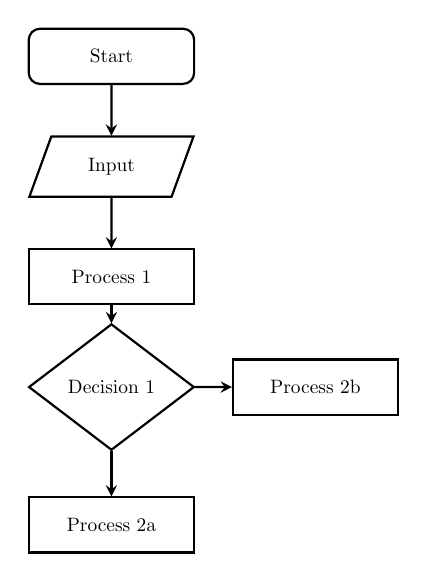
\begin{tikzpicture}[thick,scale=0.7, every node/.style={scale=0.7},node distance=2cm]
%Calling the blocks
\node (start) [startstop] {Start};
\node (in1) [io, below of=start] {Input};
\node (pro1) [process, below of=in1] {Process 1};
\node (dec1) [decision, below of=pro1] {Decision 1};
\node (pro2a) [process,below of= dec1,yshift = -0.5cm]{Process 2a};
\node (pro2b) [process, right of = dec1,xshift = 1.7cm] {Process 2b};
% Drawing the arrows between blocks
\draw[arrow] (start) -- (in1);
\draw[arrow] (in1) -- (pro1);
\draw[arrow] (pro1) -- (dec1);
\draw[arrow] (dec1) -- (pro2a);
\draw[arrow] (dec1) -- (pro2b);
\end{tikzpicture}
\caption{General Flowchart}
\label{fig:flowchart}
\end{figure}




\end{document}






